\chapter{Background}
This chapter contains two main topics. Firstly, it gives the description of Multi Quality Auto Tunning (MQuAT) and later gives the basic concept of genetic algorithms, it's components.

\section{Multi Quality Auto Tunning (MQuAT)}
here will be information about MQuAT
\subsection{MQuAT problem}

MQuAT problem
     
\section{Genetic algorithm}
Evolutionary algorithms is a subset of evolutionary computation and belongs to set of modern heuristics based search method.
\todo{Vikhar, P. A. "Evolutionary algorithms: A critical review and its future prospects". Proceedings of the 2016 International Conference on Global Trends in Signal Processing, Information Computing and Communication (ICGTSPICC). Jalgaon, 2016, pp. 261-265. ISBN 978-1-5090-0467-6.}
Appeared as a result of the influence the biological evolution on computer scientists. This domain contains different types.
There are
\begin{itemize}
	\item Genetic algorithm 
	\item Genetic programming
	\item Evolutionary programming
	\item Evolution strategy
\end{itemize}

Genetic algorithm (GA) is the most popular type of EA.

\begin{figure}
	\centering
	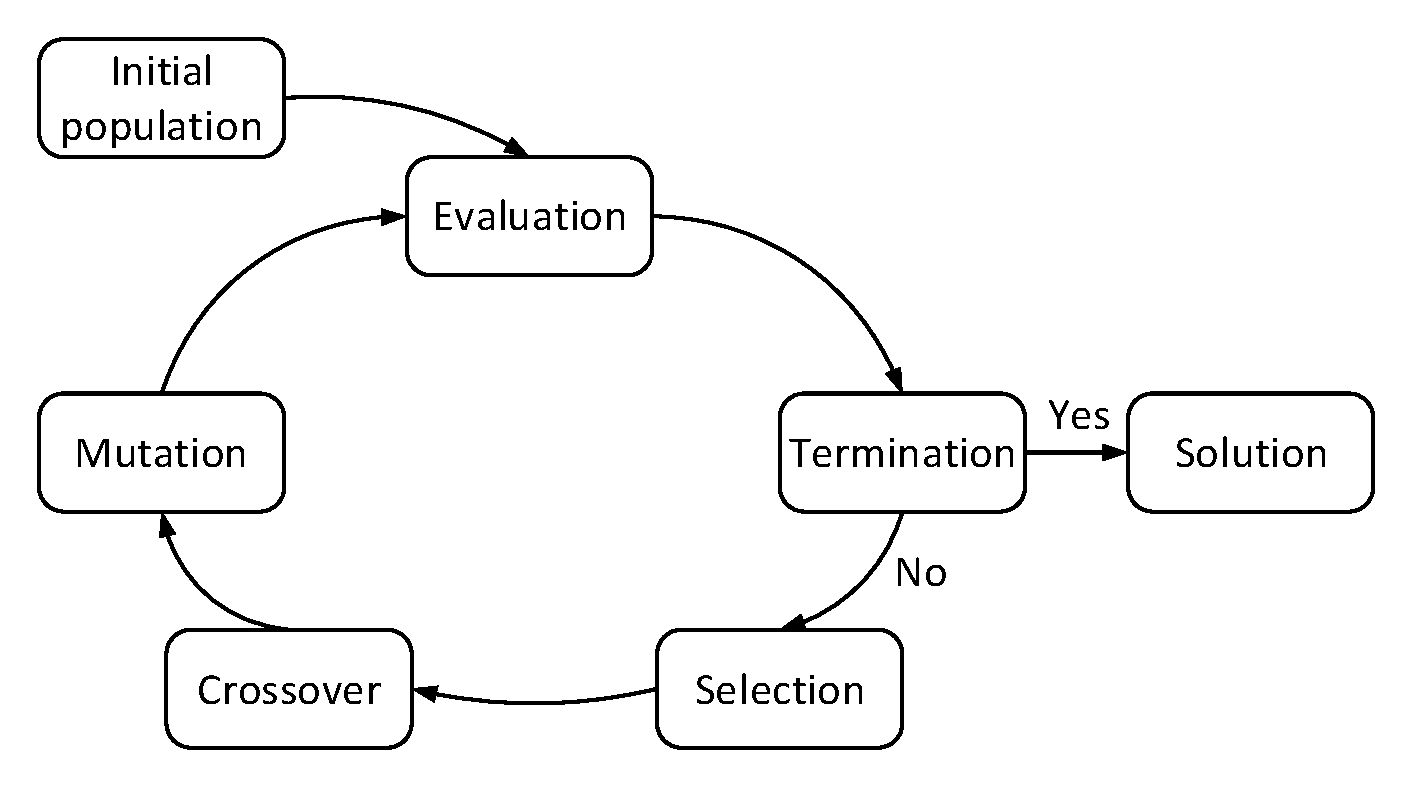
\includegraphics{images/GeneticLoop}
	\caption{Main loop of the genetic algorithm}\label{fig:example}???
\end{figure}
Main principle of GA looks like a loop with several steps.
First step is creation of initial population - a set of randomly created individuals each of them represent one solution. 
Second step is Evaluation. Calculate fitness or objective function of current population.
If solution is founded and all requirements for the termination are fulfilled then we will get the final solution. Otherwise, select best candidates to create new generation.
In step 4 using recombination and mutation on selected candidates GA creates new generation of population. And after that evaluate it.

GA based on different components and operators.
\subsection{Selector}
Selector is one of the most important components of GA. It selects \textit{mu} number of individuals from the population. The motivation of this operation come from Charles Darwin's theory of natural selection. He says that the most fitted or adapted individuals have a better chance to get better offspring.

There are many different selection algorithms
\begin{itemize}
	\item NSGA2 (Non-dominated sorting based genetic algorithm)
	\item SPEA2 (Strength Pareto Evolutionary Algorithm)
	\item NSGA3\todo{litref}
	\item SPEA3\todo{litref}
	\item PDE \todo{litref}
\end{itemize}
In this thesis we will focus on selection algorithm only as a parameter of genetic algorithm and will use NSGA2 and SPEA2. 
\todo{Do I need to describe how works NSGA2 and SPEA2?}
\subsection{crossover}
Crossover is an operator of genetic algorithm that allows recombination of two individuals by swapping some genes between them.
In general, crossover has a several parameters such as
\begin{itemize}
	\item Crossover rate - parameter that describes the probability of two chromosomes to exchange their genes.
	\item Crossover point - the point in which the exchange could be done.
\end{itemize}

The principle of the crossover is next.
Firstly, select the crossover point. For example, chromosome could be described as a vector of bits, then the crossover point will be the start index of bits which will be replaced from another chromosome.
Secondly, swap genes between chromosomes.

\todo{fig}

\subsection{mutation}

Mutation is an operator of genetic algorithm that change single gene in a chromosome. As a crossover operator, mutation has parameters:

\begin{itemize}
	\item Mutation rate - parameter that describes the probability mutation.
\end{itemize}

To perform mutation on chromosome need to do:
\begin{enumerate}
	\item Randomly select gene which will mutate
	\item Change selected gene to another.
\end{enumerate}

On the \todo{fig} presented simple mutation on chromosome that described as a vector of bits.

\todo{fig}

\section{Genetic solver}
To solve MQuAT problem using genetic algorithm genetic solver was developed by Jamal Ahmad.\todo{add ref to diploma} And further improved by Johannes Mey.

This solver is based on Opt4J\todo{link to website} framework. It's an open-source framework that gives the opportunity to implement genetic algorithm for custom optimization problem by specifying several modules and classes.

To solve custom problem using genetic algorithm user need to create several things:
\begin{enumerate}
	\item Creator
	\item Decoder
	\item Evaluator
\end{enumerate}
Also, if your genotype can't be described as vector, then you firstly need to implement:
\begin{enumerate}
	\item Genotype
	\item Crossover operator
	\item Mutation operator
\end{enumerate}

\subsection{Tree Shape Genotype}
Because of problem model of MQuAT in genetic solver was created Tree Shape Genotype\todo{add ref to diploma}.

\todo{will add more}.
 
\subsection{Crossover operator}
This operator perform crossover between two Tree Shaped Genotypes. 

\todo{fig}



\subsection{Mutation operator}
This operator perform crossover between two Tree Shaped Genotypes. 

\todo{fig}

\subsection{Creator}
\label{subsec:Creator}
As mentioned in Chpter1~\ref{subsec:Creator}, Genetic algorithm uses creator to create random genotypes for initial population.
In genetic solver Creator create the genotype by creating random solution model and transform it to Three Shape Genotype structure.

\todo{fig}

\subsection{Decoder}

Decoder decode genotype into phenotype.
Phenotype is a solution that could be evaluated.
In genetic solver decoder transform genotype to Solution Model of MQuAT.

\todo{fig}

\subsection{Evaluator}

Evaluator calculate objective functions of the solution. 
In genetic solver the evaluator calculates two \todo{or three?} objectives:

\begin{enumerate}
	\item Validity errors - number of violated contracts
	\item Energy value - energy consumption
\end{enumerate}









